\documentclass[11pt,a4paper]{article}
\usepackage{graphicx} 
\usepackage{multirow}
\usepackage{enumitem}
\usepackage{amssymb}
\usepackage{amsmath}
\usepackage{amsthm}
\usepackage{xcolor}
\usepackage{tikz}
\usepackage{tikz-3dplot}
\usepackage{pgfplots}
  \pgfplotsset{
        every non boxed x axis/.style={
            xtick align=center,
            tick style={line width=0.5pt, color=black},
            x axis line style={-{Latex[width=1.5mm]},black,line width=0.5pt},
            xlabel style={at={(ticklabel* cs:1.05)}, anchor=mid},
            xlabel=$x$
        },
         every non boxed y axis/.style={
            ytick align=center,
            tick style={line width=0.7pt, color=black},
            y axis line style={-{Latex[width=1.5mm]},black,line width=0.5pt},
            ylabel style={at={(ticklabel* cs:1.08)}, anchor=mid},
            ylabel=$y$
        },
        every non boxed z axis/.style={
            ztick align=center,
            tick style={line width=0.5pt, color=black},
            z axis line style={-{Latex[width=1.5mm]},black,line width=0.5pt},
            zlabel style={at={(ticklabel* cs:1.06)}, anchor=mid},
            zlabel=$z$
        },
        tick label style={
            font=\tiny,
        },
        compat=1.18
    }

  \usepgfplotslibrary{colormaps,patchplots}
  \usepgfplotslibrary{fillbetween}
  \pgfplotsset{colormap={cm}{color(0)=(cyan) color(1)=(cyan!90) color(3)=(cyan!80) color(4)=(cyan!70) color(5)=(cyan!10)}}
  \usetikzlibrary{arrows.meta}
\usepackage{geometry}
	\geometry{
		total = {160mm, 237mm},
		left = 20mm,
		right = 20mm,
		top = 20mm,
		bottom = 20mm,
	}
\usepackage{hyperref}
\hypersetup{
    colorlinks=true,
    linkcolor=blue,
    filecolor=magenta,      
    urlcolor=cyan,
    pdftitle={Overleaf Example},
    pdfpagemode=FullScreen,
    }
\usepackage{fancyhdr}
\renewcommand{\headrulewidth}{0pt}
\renewcommand{\arraystretch}{1.1}
\pagestyle{fancy}

\graphicspath{{C:/Users/teoso/OneDrive/Documents/Tugas Kuliah/Template Math Depart/}{D:/Hada Touya/Tugas-Kuliah/Template Math Depart/}}

\newcommand{\R}{\mathbb{R}}
\newcommand{\N}{\mathbb{N}}
\newcommand{\Z}{\mathbb{Z}}
\newcommand{\Q}{\mathbb{Q}}
\newcommand{\jawab}{\textbf{Solusi}:}

\newtheorem*{teorema}{Teorema}
\newtheorem*{definisi}{Definisi}


\begin{document}
\begin{table}[h!]
  \centering
  \begin{tabular}{|r c|}
    \hline
    \multicolumn{2}{|c|}{\MakeUppercase{\large\bfseries evaluasi tengah semester gasal 2024/2025}}                         \\
     &                                                                                                                     \\
    \begin{tabular}{c}
      \includegraphics[width=2cm]{ITS.png}
      \includegraphics[width=2cm]{M.png}      \\
      {\large\bfseries Departemen Matematika} \\
      {\large\bfseries FSAD}
    \end{tabular}
     & \begin{tabular}{lcll}
         Matakuliah    & : & \multicolumn{2}{l}{Kalkulus Peubah Banyak}                                              \\
         Hari, Tanggal & : & \multicolumn{2}{l}{Selasa, 10 Desember 2024}                                            \\
         Waktu / Sifat & : & \multicolumn{2}{l}{100 menit / \textit{Tertutup}}                                       \\
         Kelas, Dosen  & : & A.                                                & Dra. Nur Asiyah, M.Si.              \\
                       &   & B.                                                & Drs. Suhud Wahyudi, M.Si.           \\
                       &   & C.                                                & Drs. Lukman Hanafi, M.Si.           \\
                       &   & D.                                                & Dr. Didik Khusnul Arif S.Si., M.Si. \\
       \end{tabular}

    \\
    \hline
    \multicolumn{2}{|l|}{\color{red}\MakeUppercase{harap diperhatikan !!!}}                                                \\
    \multicolumn{2}{|l|}{\color{red}Segala jenis pelanggaran (mencontek, kerjasama, dsb) yang dilakukan pada saat ETS/EAS} \\
    \multicolumn{2}{|l|}{\color{red}akan dikenakan sanksi pembatalan matakuliah pada semester yang sedang berjalan.}       \\
    \hline
  \end{tabular}
\end{table}

\begin{enumerate}
  \item Hitung integral berikut ini $\iiint_R dx\,dy\,dz$, dengan $R$ adalah daerah integrasi yang dibatasi oleh bidang-bidang $z=\frac{1}{2}x,\, z=0,\, y=x,\, x+y=2,$ dan $y=0$. Sketsa batas integrasi $R$.
  \item Dapatkan Volume benda yang dibatasi $z=y$, $y=x^2$, dan $x=y^2$ yang berada dalam oktan pertama. Sketsalah batas permukaan benda tersebut.
  \item Gambarkan keping datar homogen yang dibatasi oleh kurva-kurva $x(1-y)=1$, $x(1-y)=2$, $xy=1$, dan $xy=3$. Hitung pula momen inersia terhadap sumbu $y$. (Petunjuk: transformasi ke koordinat baru $(u,v)$)
  \item Dapatkan pusat massa permukaan benda $2z=8-x^2-y^2$, jika densitinya konstan, yang berada dalam silinder $x^2+y^2=3$. Sertai dengan sketsa permukaan benda.
\end{enumerate}
\vspace*{1cm}
\begin{center}
  \textbf{Selamat Mengerjakan Semoga Sukses}
\end{center}
\newpage
\fancyhead[L]{\textit{Solution By: \hyperlink{https://github.com/TetewHeroez}{Tetew}}}
\fancyfoot[C]{}
{\centering
  \textbf{SOLUSI}
  \par
}
\begin{enumerate}
  \item Pertama-tama agar lebih mudah dalam mengilustrasikan batas-batas bidang, dapat kita gambar sketsa batas integrasi $R$ di bidang $xy$ terlebih dahulu. Dibawah ini adalah sketsa untuk batas-batas $y=0$, $y=x$, dan $x+y=2$.
        \begin{center}
          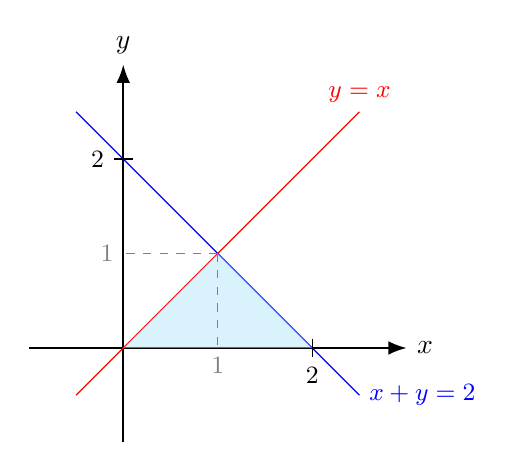
\begin{tikzpicture}[scale=1.2]
            \draw[-Latex,thick] (-1,0) -- (3,0) node[right] {$x$};
            \draw[-Latex,thick] (0,-1) -- (0,3) node[above] {$y$};
            \draw[blue,domain=-0.5:2.5] plot (\x, {2 - \x}) node[right] {\small$x+y=2$};
            \draw[red,domain=-0.5:2.5] plot (\x, {\x}) node[above] {\small$y=x$};
            \fill[cyan!30, opacity=0.5] (0,0) -- (1,1) -- (2,0) -- cycle;
            \draw[thin] (2,0.1) -- (2,-0.1) node[below] {\small$2$};
            \draw[thin] (0.1,2) -- (-0.1,2) node[left] {\small$2$};
            \draw[thin,dashed,black!50] (1,1) -- (1,0) node[below] {\small$1$};
            \draw[thin,dashed,black!50] (1,1) -- (0,1) node[left] {\small$1$};
          \end{tikzpicture}
        \end{center}
        Jadi untuk bidang-$xy$, batas-batasnya (dipilih yang termudah untuk diintegralkan) adalah $y \leq x \leq 2-y$ dan $0 \leq y \leq 1$.

        Selanjutnya ketika kita buat bangun ruang nya yang berpotongan dengan bidang $z=\frac{1}{2}z$, berikut adalah sketsa batas integrasi $R$.
        \begin{center}
          \tdplotsetmaincoords{70}{120}

          \begin{tikzpicture}[tdplot_main_coords, scale=2]

            % Sumbu koordinat
            \draw[-Latex] (0,0,0) -- (2.5,0,0) node[anchor=north east] {$x$};
            \draw[-Latex] (0,0,0) -- (0,2,0) node[anchor=west] {$y$};
            \draw[-Latex] (0,0,0) -- (0,0,1) node[anchor=south] {$z$};

            % Titik-titik pada bidang z=0 (proyeksi di bidang xy)
            % A = (0,0), B = (2,0), C = (1,1)
            \coordinate (A) at (0,0,0);
            \coordinate (B) at (2,0,0);
            \coordinate (C) at (1,1,0);

            % Segitiga dasar di bidang z=0
            \draw[thick] (A) --  (B);
            \draw[thick] (A) --  (C);
            \draw[thick] (B) --  (C);

            % Titik-titik pada bidang z = x/2
            % z = x/2: Btop = (2,0,1), Ctop = (1,1,0.5)
            \coordinate (Btop) at (2,0,1);
            \coordinate (Ctop) at (1,1,0.5);

            % Garis vertikal (sejajar sumbu z) dari dasar ke bidang z = x/2
            \draw[dashed] (B) -- (Btop);
            \draw[dashed] (C) -- (Ctop);

            % Garis-garis pada bidang z = x/2
            \draw[thick] (A) -- (Btop);
            \draw[thick] (A) -- (Ctop);
            \draw[thick] (Btop) -- (Ctop);

            % (Opsional) Arsiran volume R
            \fill[cyan,opacity=0.10] (A) -- (B) -- (C) -- cycle;          % dasar
            \fill[cyan,opacity=0.10] (A) -- (Btop) -- (Ctop) -- cycle;    % sisi miring atas
            \fill[cyan,opacity=0.05] (B) -- (C) -- (Ctop) -- (Btop) -- cycle; % sisi samping

            % Label daerah R
            \node[blue!30!cyan] at (1,0.4,0) {$R$};

            % \draw[cyan,domain=0:3] plot (\x, 0, {\x/2}) node[left] {\small$z=\frac{1}{2}x$};
            % \foreach \y in {0,0.1,...,2} {
            %     \draw[cyan,domain=0:3] plot (\x, \y, {\x/2});
            %   }
          \end{tikzpicture}
        \end{center}
        Sehingga integral yang diminta dapat dituliskan sebagai berikut.
        \begin{align*}
          \iiint_R dx\,dy\,dz & = \int_{0}^{1}\int_{y}^{2-y}\int_0^{\frac{1}{2}x} dz\,dx\,dy              = \int_{0}^{1}\int_{y}^{2-y} \left[ z \right]_0^{\frac{1}{2}x} dx\,dy    = \int_{0}^{1} \left[ \frac{1}{4}x^2 \right]_{x=y}^{x=2-y} dy                                                                                                                                                                                                                                              \\
                              & = \int_{0}^{1} \left( \frac{1}{4}(2-y)^2 - \frac{1}{4}y^2 \right) dy                                                                                                                                              = \int_{0}^{1} \left( \frac{1}{4}(4 - 4y + y^2 - y^2) \right) dy                                                                                                                                                  = \int_{0}^{1} (1 - y) dy \\
                              & = \left[ y - \frac{1}{2}y^2 \right]_0^1 = 1 - \frac{1}{2} = \frac{1}{2}.
        \end{align*}
  \item Batas permukaan di bidang-$xy$ dibatasi oleh $y=x^2$ dan $x=y^2$ di oktan pertama.
        \begin{center}
          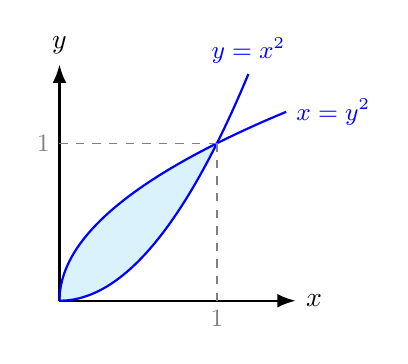
\begin{tikzpicture}[scale=2]
            \draw[-Latex,thick] (0,0) -- (1.5,0) node[right] {$x$};
            \draw[-Latex,thick] (0,0) -- (0,1.5) node[above] {$y$};
            \fill[cyan!30,opacity=0.5,domain=0:1,smooth,thick] plot (\x, {\x^2}) -- cycle;
            \fill[cyan!30,opacity=0.5,domain=0:1,smooth,thick] plot ({\x*\x}, {\x}) -- cycle;
            \draw[blue,domain=0:1.2,smooth,thick] plot (\x, {\x^2}) node[above] {\small$y=x^2$};
            \draw[blue,domain=0:1.2,smooth,thick] plot ({\x*\x}, {\x}) node[right] {\small$x=y^2$};
            \draw[thin,dashed,black!50] (1,1) -- (1,0) node[below] {\small$1$};
            \draw[thin,dashed,black!50] (1,1) -- (0,1) node[left] {\small$1$};
          \end{tikzpicture}
        \end{center}
        Dari gambar di atas dapat kita lihat bahwa batas-batasnya adalah $x^2 \leq y \leq \sqrt{x}$ dan $0 \leq x \leq 1$.

        Untuk batas permukaan atasnya adalah $0 \leq z \leq y$. Maka volume benda yang diminta adalah
        \begin{align*}
          V & = \int_{0}^{1} \int_{x^2}^{\sqrt{x}} \int_0^y dz\,dy\,dx = \int_{0}^{1} \int_{x^2}^{\sqrt{x}} \left[ z \right]_0^y dy\,dx = \int_{0}^{1} \int_{x^2}^{\sqrt{x}} y\,dy\,dx = \int_{0}^{1} \left[ \frac{1}{2}y^2 \right]_{y=x^2}^{y=\sqrt{x}} dx \\
            & = \int_{0}^{1} \left( \frac{1}{2}x - \frac{1}{2}x^4 \right) dx = \left[ \frac{1}{4}x^2 - \frac{1}{10}x^5 \right]_0^1 = \frac{1}{4} - \frac{1}{10} = \frac{3}{20}.
        \end{align*}

  \item Agar lebih mudah dalam memahami persamaan kurva, dapat kita ubah persamaan kurva tersebut menjadi bentuk $y=f(x)$. Sehingga diperoleh
        \begin{itemize}
          \item $x(1-y)=1\implies y=1-\dfrac{1}{x}$
          \item $x(1-y)=2\implies y=1-\dfrac{2}{x}$
          \item $xy=1\implies y=\dfrac{1}{x}$
          \item $xy=3\implies y=\dfrac{3}{x}$
        \end{itemize}
        Berikut adalah sketsa daerah yang dibatasi oleh keempat kurva tersebut.
        \begin{center}
          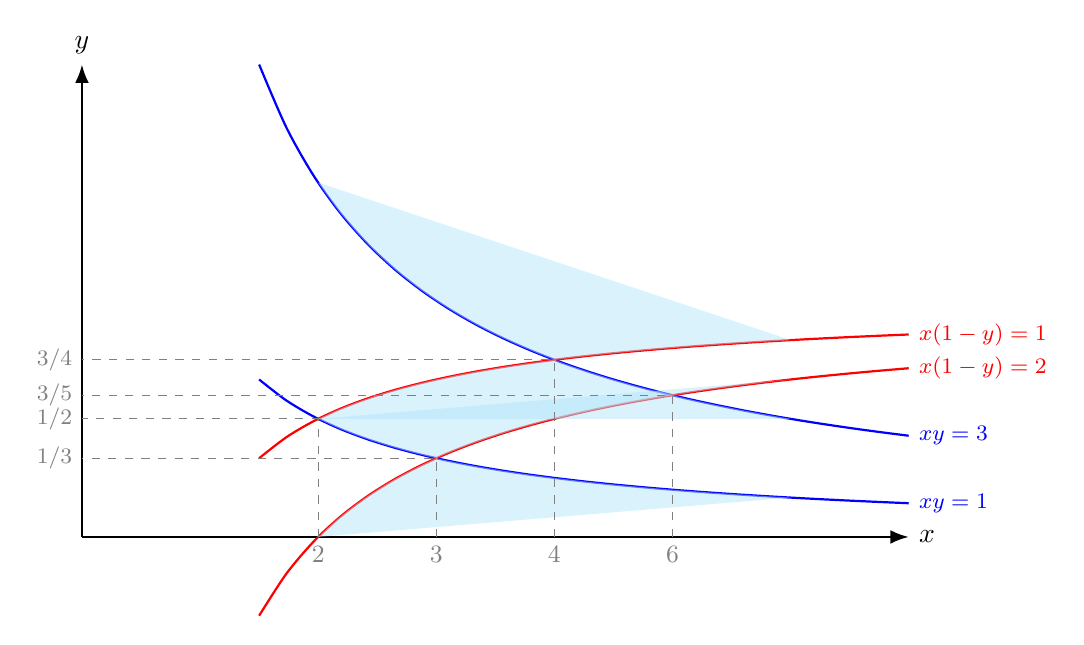
\begin{tikzpicture}[xscale=1.5,yscale=3]
            \draw[-Latex,thick] (0,0) -- (7,0) node[right] {$x$};
            \draw[-Latex,thick] (0,0) -- (0,2) node[above] {$y$};
            \draw[blue,domain=1.5:7,smooth,thick] plot (\x, {1/\x}) node[right] {\footnotesize$xy=1$};
            \draw[blue,domain=1.5:7,smooth,thick] plot (\x, {3/\x}) node[right] {\footnotesize$xy=3$};
            \draw[red,domain=1.5:7,smooth,thick] plot (\x, {1-(1/\x)}) node[right] {\footnotesize$x(1-y)=1$};
            \draw[red,domain=1.5:7,smooth,thick] plot (\x, {1-(2/\x)}) node[right] {\footnotesize$x(1-y)=2$};
            \fill[cyan!30,opacity=0.5,domain=2:6,smooth,thick] plot (\x, {1/\x}) -- plot (\x, {1-(2/\x)}) -- cycle;
            \fill[cyan!30,opacity=0.5,domain=2:6,smooth,thick] plot (\x, {1-(1/\x)}) -- plot (\x, {3/\x}) -- cycle;
            \draw[thin,dashed,black!50] (2,0) node[below] {\small$2$} -- (2,0.5) -- (0,0.5) node[left] {\footnotesize$1/2$};
            \draw[thin,dashed,black!50] (4,0) node[below] {\small$4$} -- (4,0.75) -- (0,0.75) node[left] {\footnotesize$3/4$};
            \draw[thin,dashed,black!50] (3,0) node[below] {\small$3$} -- (3,0.333) -- (0,0.333) node[left] {\footnotesize$1/3$};
            \draw[thin,dashed,black!50] (5,0) node[below] {\small$6$} -- (5,0.6) -- (0,0.6) node[left] {\footnotesize$3/5$};
          \end{tikzpicture}
        \end{center}
  \item
\end{enumerate}
\end{document}